% Tutto quello riguardante il progetto andrà in questo capitolo

\chapter{Il progetto}
\label{cap:progetto}

\section{I ricordi}

La vita di ogni persona è composta da ricordi. Sempre più oggi giorno la gente
salva i propri istanti tramite i \textit{social network}, come ad esempio
Facebook o Instagram. Ma questi momenti tendono a svanire col tempo o possono
perdersi nella vastità di internet. Quello che PastBook offre è la
possibilità di renderli permanenti in un album fotografico prendendo i momenti
salvati nei \textit{social network}. Questa operazione è resa ancora più
semplice se il tutto è assistito da un \textit{bot}, che rende il processo più e
\textit{user-friendly}.

\subsection{L'era dei \textit{bot}}

Dal lancio iniziale sulla piattaforma di messaggistica di Telegram dei
\textit{bot}, si è potuto notare come ci sia stato un maggior interessamento
verso questa tecnologia. L'entrata di Facebook tramite la sua applicazione di
messaggistica Messenger ha segnato un importante passo anche nel modo in cui le
aziende possono interagire con i propri clienti. È ora possibile scrivere
direttamente alle pagine dei servizi a cui si è interessati per ottenere aiuto o
informazioni in pochi secondi, facendo risparmiare agli utenti la fatica di
andarsele a cercare nel sito della compagnia.

%https://www.microsoft.com/cognitive-services/en-us/language-understanding-intel
%igent-service-luis
%https://wit.ai/
Questo ha fatto spingere i grandi colossi come Microsoft e Facebook stessa a
investire verso la branchia dell'intelligenza artificiale, per poter dare
alle macchine la possibilità di interpretare al meglio il linguaggio naturale
degli esseri umani.

\section{PastBot}

\begin{figure}[H]
  \centering
  
\includegraphics[scale=0.2]{PastBotLogoLong}
  \caption{Logo di PastBot}
\end{figure}
Appena uscita la possibilità di creare \textit{bot} su Facebook e collegarli
alle pagine delle aziende PastBook si è subito attivata per creare il suo
\textit{bot} che aiuti le persone nella creazione degli album in maniera
interattiva rendendo facile il loro acquisto in seguito. Questo permette anche
agli utenti la creazione e acquisto di album comodamente e direttamente da
Facebook.

Una volta arrivato nella pagina della società, l'utente non deve far altro che
scrivergli un messaggio. Al primo messaggio si attiverà il \textit{bot} che
gli risponderà cortesemente illustrandogli le sue funzionalità e comandi.
L'utente potrà chiedere aiuto al \textit{bot}, che lo guiderà nei passi
necessari per creare un album. Quando finalmente l'utente ha inviato il numero
minimo delle foto necessarie per creare l'album, verrà informato da PastBot che
gli offrirà la possibilità di acquistarlo. Questo porterà l'utente in una
procedura automatica di acquisto, in cui gli unici campi richiesti saranno
solamente selezionare il tipo di pagamento, la località dove spedire il libro
dei ricordi appena creato e in che formato lo si desidera. \\

Essendo l'utente un essere umano si è dovuto considerare dei possibili errori
che esso può commettere:
\begin{itemize}
  \item errori in fase di digitazione;
  \item errori nell'invio delle immagini;
  \item errori nell'interpretazione dei messaggi del \textit{bot}.
\end{itemize}

\paragraph*{Errori di digitazione} Per gli errori di digitazione il \textit{bot}
segnalerà all'utente l'eventuale errore (se l'errore si trova nella parola
chiave del comando), chiedendogli di effettuare di nuovo l'operazione richiesta.

\paragraph*{Errori nell'invio delle immagini} Durante l'invio delle immagini, è
possibile che l'utente possa commettere un errore nella selezione e possa
inviare anche altri contenuti, come file generici o video. In questo caso, il
\textit{bot} ignorerà i contenti diversi da immagini che sono stati inviati,
senza lanciare un messaggio di errore o fermare l'operazione di caricamento.
Questa scelta è stata presa in quando è possibile che questo tipo di errore
avvenga maggiormente quando l'utente vuole inviare un gran numero di foto nella
chat, ed eseguire azioni come segnalare l'errore o fermare il processo di
salvataggio delle immagini potrebbe portare a reazioni come frustrazione e
fastidio.

\paragraph*{Errori di interpretazioni} È anche possibile che le persone
commettano degli errori nell'interpretare il senso della frase che il
\textit{bot} manda loro. Questo potrebbe portare a un errore nella procedura
richiesta dal \textit{bot}. Un tipico esempio potrebbe essere richiedere la
lista delle foto di un album che è attualmente vuoto. In questo caso il
\textit{bot} segnalerà all'utente che l'azione non è disponibile, e provvederà
a fornirgli una lista di azioni che può intraprendere. In questa maniera si
inviterà a continuare attivamente la conversazione.

\begin{figure}[H]
  \centering
  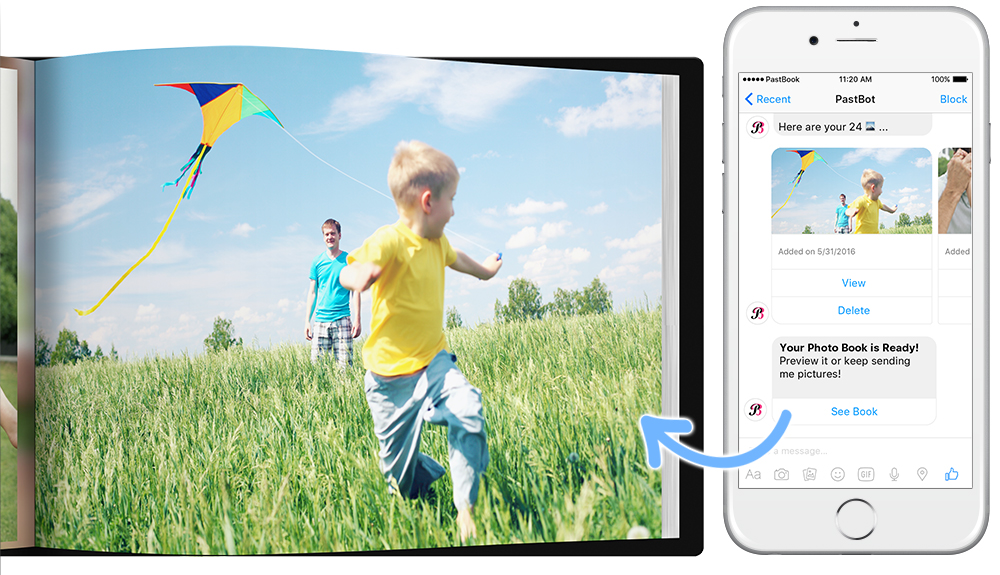
\includegraphics[scale=0.35]{PastBotLandingPage}
  \caption{Presentazione del bot all'utenza finale}
\end{figure}

\subsection{Azioni intraprendibili dall'utente}

L'utente può intraprendere con PastBot diversi tipi di azioni. Di seguito si
elencano le possibili:

%magari è meglio usare una tabella qui?
\begin{itemize}

  \item richiedere informazioni riguardo al funzionamento del \textit{bot};
  \item richiedere informazioni riguardo ai costi di spedizione e ai formati
degli album;
  \item creare un nuovo album;
  \item inviare foto al \textit{bot} tramite la chat utente;
  \item vedere la lista delle foto inviate e attualmente presenti all'interno
dell'album;
  \item richiedere di vedere, a grandezza originale e senza alcuna riduzione di
risoluzione un'immagine presente nella lista dell'album che si sta creando;
  \item richiedere di cancellare una specifica foto dall'album che si sta
creando;
  \item procedere con l'acquisto dell'album.
\end{itemize}

\subsection{Implementazione tecnica}

\subsubsection{Amazon AWS Lambda}
%https://aws.amazon.com/lambda/
\begin{figure}[H]
  \centering
  
\includegraphics[scale=0.08]{LambdaLogo}
  \caption{Logo di Amazon AWS Lambda}
\end{figure}
PastBook basa i suoi servizi nel \gls{cloud} grazie a Amazon AWS Services.
Per realizzare il \textit{bot} è quindi stato deciso di pensarlo utilizzando
un'architettura \glslink{serverless}{serverless} con database non relazionali
(ovvero di tipo \glslink{nosql}{NoSQL}). Un'architettura di questo tipo porta a
diversi vantaggi:

\begin{itemize}

  \item nessun costo di amministrazione dei server in cui il programma viene
eseguito;
  \item l'applicazione ha la possibilità di scalare in automatico in base alle
richieste in arrivo, per offrire un servizio all'utenza senza interruzioni;
  \item i costi sono legati solamente al tempo di esecuzione effettivo del
programma nel \gls{cloud};
  \item risorse automaticamente gestite;
  \item reigstrazione automatica degli eventi dell'applicazione;
  \item raccolta automatica di metriche e statistiche sull'utilizzo delle
risorse;
  \item tutto l'ambiente è all'interno dello stesso \gls{cloud}, permettendo
una comunicazione interna molto rapida e riducendo i tempi di chiamate delle
varie \gls{api}.
\end{itemize}

Questo tipo di vantaggi ha permesso anche durante il tirocinio di focalizzarsi
prevalentemente nella stesura del codice senza preoccuparsi della parte di
amministrazione del sistema.

Il servizio \gls{cloud} utilizzato nello specifico si chiama Amazon AWS
Lambda, e permette di configurare quante risorse per quanto tempo il programma
potrà avere.
AWS Lambda permette di caricare il codice sotto forma di "funzioni". Queste
funzioni non sono altro che porzioni di codice (che possono essere composte da
più file).
Nella configurazione sarà poi necessario definire il metodo della
"funzione" da invocare al sopraggiungere di una richiesta. A questa funzione
verrà passato un evento sotto forma di oggetto
\glslink{javascript_object_notation}{JSON}. I campi per l'oggetto sono
definibili e personalizzabili nella configurazione della funzione, oppure si può
scegliere di ricevere tutti i campi dell'evento.
Per poter automatizzare anche questa configurazione, creando
quindi un sistema completamente automatizzato per la distribuzione del
codice, si è deciso di utilizzare lo strumento open source Apex.

\subsubsection{Apex}
% http://apex.run/
\begin{figure}[H]
  \centering
  
\includegraphics[scale=0.5]{ApexLogo}
  \caption{Logo di Apex}
\end{figure}

Apex è uno strumento che permette di automatizzare la fase di distribuzione del
codice sorgente con configurazioni personalizzabili in base all'ambiente in cui
si distribuisce il programma. Oltre a queste funzionalità, permette anche di:
\begin{itemize}
  \item eseguire la funzione direttamente da linea di comando (il codice verrà
comunque eseguito in remoto);
  \item visualizzazione di metriche sull'utilizzo del programma;
  \item visualizzazione dei registri di esecuzione.
\end{itemize}

Per utilizzare questo strumento è stato necessario creare la struttura del
progetto secondo quanto specificato dalla documentazione del programma.

\paragraph*{Struttura di un progetto Apex}

\begin{figure}[H]
  \centering
  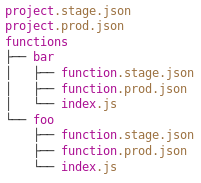
\includegraphics[scale=0.7]{project_structure}
  \caption{Tipica struttura di un progetto Apex}
\end{figure}

% http://apex.run/#structuring-projects
Come è possibile notare nella figura, sono presenti diversi file di
configurazione di tipo \glslink{javascript_object_notation}{JSON}. Prima
dell'estensione del file è possibile notare come siano appuntati i vari tipi di
environment, per cui è possibile creare una configurazione diversa.
All'interno del file "project.<environment>.json" è possibile inserire i
seguenti campi:
\begin{itemize}
  \item \textbf{name}: il nome del progetto;
  \item \textbf{description}: una descrizione del progetto (questo campo può
essere opzionale);
  \item \textbf{runtime}: specifica ad Apex il tipo di linguaggio e la versione
dell'interprete per il linguaggio scelto che è necessario utilizzare. Le
versioni attualmente supportate dallo strumento sono maggiori di quelle che
permette il servizio Amazon Lambda, che è limitato solamente ai linguaggi come
JavaScript, Python e Java. Le opzioni disponibile per questo campo sono:
  \begin{itemize}
    \item java (utilizzo di Java versione 8)
    \item python (versione 2.7)
    \item nodejs (versione 0.10)
    \item nodejs4.3 (versione 4.3)
    \item golang (qualsiasi versione)
  \end{itemize}

  \item \textbf{memory}: la memoria che le varie macchine Lambda disporranno.
La memoria utilizzabile varia da un minimo di 128 MB di RAM fino a un massimo
di 1536MB di RAM. Questo campo richiede l'inserimento di un valore intero;

  \item \textbf{timeout}: indica il tempo massimo di esecuzione della singola
funzione Lambda: infatti è possibile che la macchina abbia dei periodi di
esecuzione più lunghi di quelli desiderati. Se l'esecuzione supera il limite
impostato, l'esecuzione della funzione verrà interrotta. Questo valore
attualmente può essere impostato a un massimo di 5 minuti;

  %http://docs.aws.amazon.com/general/latest/gr/aws-arns-and-namespaces.html
  \item \textbf{role}: all'interno dell'ambiente Amazon AWS sono presenti i
ruoli, che danno la possibilità di definire i permessi delle varie risorse
all'interno del servizio, siano essi utenti della compagnia o servizi in
esecuzione. Ogni permesso è identificato tramite un \textit{Amazon Resource
Names} (anche abbreviato in ARN), che segue la seguente definizione:
\begin{verbatim}
  arn:partition:service:region:account-id:resource
\end{verbatim}
dove:
  \begin{itemize}
    \item[arn] identifica che si tratta di un ruolo;

    \item[partition] indica il tipo di luogo in cui si trova la risorsa.
Attualmente è solamente disponibile il valore "aws";

    \item[service] indica il servizio. Nel caso della configurazione necessaria
per il tirocinio, il valore è stato impostato a "lambda";

    \item[region] indica la regione dove questa risorsa è allocata. Amazon AWS
Services è un servizio presente in più regioni del mondo, e ogni regione
permette di avere una propria configurazione;

    \item[account-id] indica l'id dell'\textit{account} con cui si sta
assegnando il permesso;

    \item[resource] è il nome della risorsa, che è univoco per quel determinato
servizio nella regione selezionata.
  \end{itemize}
  L'assegnazione di un ruolo è obbligatorio e se non correttamente configurato
durante l'esecuzione del codice si potrebbero riscontrare problemi con i
permessi.

  \item \textbf{name-template}: questo campo indica il nome che la funzione
avrà quando sarà caricata nel servizio Amazon Lambda. Questo nome infatti può
essere personalizzato usando delle sequenze predefinite. Seguendo le
convenzioni stabilite all'interno di PastBook, il nome è stato definito in
questa maniera:
\begin{verbatim}
  {{.Project.Environment}}-{{.Function.Name}}
\end{verbatim}
Dove nella prima parte sarà il tipo di ambiente in cui verrà caricata la
funzione (ovvero o \textit{dev} o \textit{qa} o \textit{prod}) mentre nella
seconda si avrà il nome della cartella che ospita il codice della funzione;

  \item \textbf{handler}: questo parametro indica il nome del metodo della
funzione che Amazon Lambda chiamerà quando ne sarà richiesta l'esecuzione.
\end{itemize}


Una volta definito il file di configurazione per il progetto è possibile
cominciare a lavorare sulle funzioni che poi verranno caricate nel servizio
Amazon Lambda. Queste funzioni devono trovarsi all'interno di una propria
cartella all'interno di "function". Il nome della cartella indicherà anche il
nome della funzione. Per ogni funzione è poi possibile scrivere il codice che
verrà eseguito.

\paragraph*{Personalizzazione delle configurazioni} Apex è uno strumento
flessibile che permette di definire in maniera dettagliata ulteriori
configurazioni per ogni funzione, tramite la definizione di un file
"\textit{function.<environment>.json}". Anche questo file è un oggetto di tipo
\glslink{javascript_object_notation}{JSON}, con gli stessi campi del file
"\textit{project.<environment>.json}": ciò permette una ridefinizione dei valori
dei campi che si vuole personalizzare per quella funzione, consentendo quindi
la creazione di una configurazione globale per tutto il progetto e una
personalizzata per ogni funzionalità.
Come convenzione interna della compagnia è stato deciso di nominare tutti i
file che vengono poi eseguiti dal servizio Lambda con il nome di
\textit{index.js}.

\subsubsection{NPM}
\begin{figure}[H]
  \centering
  
\includegraphics[scale=0.08]{NpmLogo}
  \caption{Logo di NPM}
\end{figure}

Il \textit{bot} durante lo sviluppo ha richiesto la
necessità di dipendenze di terze parti, e per questo è stato deciso di
integrarle tramite il gestore di moduli JavaScript NPM.

NPM è un acronimo per Node Package Manager, e provvede a fornire una serie di
moduli creati da altri utenti. Questi moduli possono instaurare delle dipendeze
tra di loro, creando un sistema in cui il riutilizzo gioca un ruolo chiave.
Questa cooperazione di pacchetti permette la creazione di altro software in
maniera più semplice.
NPM offre anche la possibilità di rendere i pacchetti privati e non
condivisibili pubblicamente, consentendo ad aziende di sviluppare codice
proprietario in moduli per riutilizzarlo per diversi progetti interni.

All'azione di caricamento, Apex riconosce la dipendenza da altri moduli
JavaScript, provvedendo quindi a generare un file .zip che li contenga tutti e
a caricarli nel servizio.

\subsubsection{Progettazione della struttura \glslink{serverless}{serverless}}
La progettazione di un'architettura di tipo \glslink{serverless}{serverless} ha
portato alla creazione di due parti principali del \textit{bot}, ovvero una
parte dedicata solamente alla ricezione dei messaggi e all'interazione con
l'utente e la rimanente per eseguire le operazioni sui database non relazionali.
% FIXME: meglio aggiungere la definizione API come voce glossario?
La parte riguardante le operazioni sui database non relazionali è stata
suddivisa ulteriormente, e ogni funzionalità è stata posta in una "funzione"
AWS Lambda apposita, in maniera tale da aver una miglior gestione delle
risorse. Si è deciso di chiamare questa parte \gls{api}. Le \gls{api} decise in
fase di progettazione sono state le seguenti:
\begin{itemize}
  \item \textbf{addPastBotMessage}: aggiunge i messaggi ricevuti nel database
ai fini di raccolta dati;

  \item \textbf{createPastBotCollection}: questa \gls{api} si occupa della
creazione di nuovi album;

  \item \textbf{createPastBotUser}: si occupa della creazione dei nuovi utenti
che scriveranno a PastBot;

  \item \textbf{deletePastBotCollectionPhoto}: si occupa della cancellazione di
una singola foto da una determinata collezione;

  \item \textbf{getPastBotCollection}: ritorna la collezione attualmente attiva
dato un id di un utente iscritto;

  \item \textbf{getPastBotUser}: ritorna tutte le informazioni attualmente
presenti su quell'utente, come la lista delle collezioni create e la lista
attualmente attiva;

  \item \textbf{putPastBotCollectionPhoto}: dato un \gls{url} di un'immagine
valido, provvede ad aggiungere quell'immagine nel database di PastBot
assegnandola all'ultima collezione di foto attiva.
\end{itemize}

Questa suddivisione tra \gls{api} e il bot che ha il compito di ricevere i
messaggi è stata determinata anche grazie al servizio Amazon AWS APIGateway.

\subsubsection{APIGateway}
\begin{figure}[H]
  \centering
  
\includegraphics[scale=0.5]{ApigatewayLogo}
  \caption{Logo di APIGateway}
\end{figure}
APIGateway è uno dei molti servizi presenti all'interno di Amazon AWS Services
e serve per la gestione e instradamento delle richieste.
Oltre a permettere la definizione e la gestione di \gls{api} in maniera
semplice mette anche a disposizione:
\begin{itemize}
  \item integrazione nativa di con tutti gli altri servizi offerti da Amazon
AWS;
  \item gestione integrata dei permessi e controllo degli accessi;
  \item monitoraggio del volume di richieste;
  \item versionamento delle \gls{api};
  \item grazie alla distribuzione del servizio in varie parti del mondo viene
assicurata una bassa latenza per prestazioni maggiori.
\end{itemize}
La definizione di un determinato \gls{url} permette di configurare l'evento ad
esso associato in base al tipo di richiesta \gls{crud}. Al momento della
definizione, è necessario selezionare quale servizio gestirà la richiesta. Ai
fini del progetto, a ogni \gls{url} è stata associata una chiamata a una
specifica funzione Lambda.

In questa maniera, tramite l'utilizzo di un gestore di \gls{api} si è potuto
definire un servizio \glslink{serverless}{serverless} ben incapsulato: infatti
chi andrà a effettuare le chiamate alle varie \gls{api} non sarà a conoscenza di
come esse sono strutturate internamente e di come esse verranno gestite.
Le \gls{api} hanno richiesto una loro definizione e una loro progettazione
prima di essere implementate su APIGateway, e per compiere questo passo si è
ricorsi allo strumento Swagger.


\subsubsection{Swagger}
\begin{figure}[H]
  \centering
  
\includegraphics[scale=0.4]{SwaggerLogo}
  \caption{Logo di Swagger}
\end{figure}
Swagger è uno strumento potente che permette la rappresentazione di \gls{api}
per il web con relativa documentazione. È utilizzabile tramite la definizione
di un file di configurazione di tipo \gls{yaml}: in questa maniera si vengono a
definire i punti d'accesso all'applicazione e se ne compie anche una loro
descrizione. È possibile definire il file di tipo \gls{yaml} tramite l'aiuto di
un apposito editor di testo.

La decisione di usare questo strumento per definire i punti d'accesso
all'applicazione è stata presa in merito al supporto nativo che il servizio
Amazon AWS APIGateway fornisce a Swagger. Quindi si è proceduti nella seguente
maniera:
\begin{enumerate}
  \item progettazione dei punti d'accesso all'applicazione;
  \item definizione dei punti d'accesso in un file Swagger;
  \item configurazione del servizio APIGateway tramite il caricamento del file
Swagger.
\end{enumerate}


L'utilizzo di un file di configurazione porta alla possibilità di
tenere il file sotto uno strumento di versionamento, e quindi di poterne avere
sempre una storia associata al progetto, inoltre, in caso ci siano problemi o
errori sarà più facile individuali essendo la definizione tutta in un unico
file, e non distribuita nell'interfaccia grafica dello strumento di comando di
APIGateway.
Il sistema di versionamento utilizzato durante il tirocinio è stato Git.


% FIXME: rivedere l'ordine di quando si parla di git, forse è meglio spostarlo
%prima
\subsubsection{Git}
\begin{figure}[H]
  \centering
  
\includegraphics[scale=0.4]{GitLogo}
  \caption{Logo di Git}
\end{figure}
Git è un sistema di versionamento, ovvero uno strumento che aiuta i
programmatori a tenere traccia delle modifiche che un file o una porzione di
codice ricevono. Utilizzare questo sistema di versionamento ha diversi vantaggi
anche a livello organizzativo, e ha permesso durante la codifica di
sperimentare diverse soluzioni ai problemi incontrati tramite l'utilizzo di
diversi rami di sviluppo. Grazie a tale strumento, si è anche potuto evitare
casi di sovrascrittura del codice, ovvero quando due programmatori vanno a
modificare una medesima porzione del programma.

A ogni versione stabile del software raggiunta nel ramo \textit{prod}, si è
deciso di rilasciare un \textit{tag}, ovvero un'etichetta che identifica in
maniera univoca quella determinata versione del codice. Così facendo, si può
avere uno storico delle versioni stabili.
% Il resto su git è già stato detto nell'introduzione

\subsubsection{DynamoDB}
\begin{figure}[H]
  \centering
  
\includegraphics[scale=0.08]{DynamoDBLogo}
  \caption{Logo di DynamoDB}
\end{figure}
DynamoDB è un altro dei servizi che Amazon AWS mette a disposizione. Questo
offre un database flessibile di tipo \glslink{nosql}{NoSQL}, per tutti
quei servizi che necessitano di poca latenza e debbano scalare in un futuro.
AWS DynamoDB è totalmente gestito da Amazon, ed è consigliato per le
applicazioni legate al mondo del web.
Ai fini di PastBot, DynamoDB è stato essenziale per salvare i messaggi, gli
utenti e gli album con le relative foto. Il trasferimento dei dati è stato
eseguito inviando direttamente oggetti di tipo
\glslink{javascript_object_notation}{JSON} al database.

\subsubsection{Messenger e Facebook}
\begin{figure}[H]
  \centering
  
\includegraphics[scale=0.4]{MessengerLogo}
  \caption{Logo di Messenger}
\end{figure}
PastBot è nato per essere integrato con le \gls{api} della piattaforma di
messaggistica istantanea Facebook Messenger.
Prima di poter cominciare a sviluppare un bot per la piattaforma Messenger è
necessario creare un'applicazione dalla sezione dedicata agli sviluppatori per
Facebook.
Una volta creata l'applicazione, è stato possibile creare un codice
identificativo univoco utilizzabile dal \textit{bot} per inviare e ricevere
contenuti.

Messenger mette a disposizione una lista selezionabile di eventi che si desidera
inviare al bot, dove gli eventi sono:
\begin{itemize}
  \item ricezione di un messaggio;
  \item pressione di un bottone o di un link dal menù permanente;
  \item ricezione di un messaggio dal bottone "Invia a Messenger";
  \item ricezione della notifica di ricezione del messaggio da parte
dell'utente;
  \item ricezione del messaggio inviato all'utente (anche detto \textit{echo}).
\end{itemize}

Le azioni eseguibili dal bot sono la notifica all'utente che si otterrà a breve
una risposta e l'invio di messaggi, che possono essere di diverso tipo:
\begin{itemize}
  \item messaggi di testo;
  \item immagini;
  \item video;
  \item immagini con risposte rapide\footnote{Le risposte rapide sono dei
bottoni presenti subito sotto il messaggio del bot, che possono aiutare
l'utente perché non è necessario digitare testo per rispondere al bot, ma è
possibile selezionare una risposta in maniera rapida.};
  \item messaggi composti da titolo, sottotitolo, un'immagine e dei bottoni
opzionali;
  \item invio di ricevute d'acquisto.
\end{itemize}

Durante lo sviluppo del \textit{bot} avere a disposizione diversi tipi di
messaggi da poter inviare si è rivelato molto utile al fine di poter creare una
maggiore interazione con l'utente e ottenere in generale un risultato migliore
e più appetibile.

L'applicazione creata è poi stata associata a una pagina di Facebook. In questa
maniera gli utenti, scrivendo alla pagina, mandano il messaggio direttamente al
bot che provvederà poi a rispondergli nella maniera adeguata.


\subsubsection{DashBot}
\begin{figure}[H]
  \centering
  
\includegraphics[scale=0.5]{DashBotLogo}
  \caption{Logo di DashBot}
\end{figure}
La compagnia ha ritenuto importante raccogliere dati sull'utilizzo del
\textit{bot} per poter offrire un servizio migliore all'utenza in futuro. Per
adempiere a questo obiettivo è stato deciso di utilizzare la piattaforma web
\textit{dashbot.io}. DashBot è un servizio web gratuito che mette a
disposizione delle \gls{api} ai programmatori dove poter inviare i messaggi
ricevuti e i messaggi che si ha intenzione di inviare. Una volta inviato il
contenuto del messaggio, il servizio si preoccuperà di analizzarne il contenuto
ed estrapolarne le informazioni sull'utente (nazionalità, sesso, lingua madre)
e sul tipo di contenuto inviato (testo o allegato). In base a questi fattori, è
in grado di creare statistiche riguardo a:
\begin{itemize}
  \item livello di intrattenimento;
  \item ritorno dell'utenza;
  \item numero di messaggi scambiati per utente;
  \item conteggio dei messaggi ricevuti e inviati;
  \item tipo di testo ricevuto;
  \item lunghezza delle sessioni di chat per utente.
\end{itemize}
I dati vengono poi mostrati tramite diversi tipi di grafici e permette di avere
una visione generale sull'utilizzo del \textit{bot} e sul suo gradimento.
